\section{Simulation Environment}
\label{sec:simulation}

\begin{outline}
  Describe the physics-based simulation environment (IsaacLab) and
  the quadruped model used for development and testing.
\end{outline}

The simulation environment used for this project is NVIDIA Isaac Lab
\cite{mittal_orbit_2023}. This was chosen for a number of reasons. It
is a modern framework with a Python interface specifically designed
for machine learning, and GPU parallelism. The GPU parallelism
enabled much faster simulation and data-collection at the cost of
more complicated programming and reduced compatibility with older
hardware. Additionally, there are a large number of example and
community projects demonstrating many of the simulation features
needed for this project.

Despite the simulation and learning being run on the GPU, the
robot controllers are run on the CPU. \autoref{fig:diagram-processing-flow}
shows a block diagram of the processing flow. The simulation
environment is run entirely on the GPU, with each robot being
simulated in parallel. The robot MPCs are run on the CPU,
with each robot controller being run in parallel. The CPU and GPU
communicate at each simulation step to exchange the robot state and
the control actions.

\begin{todo}
  add in learning step
\end{todo}

\begin{figure}[H]
  \centering
  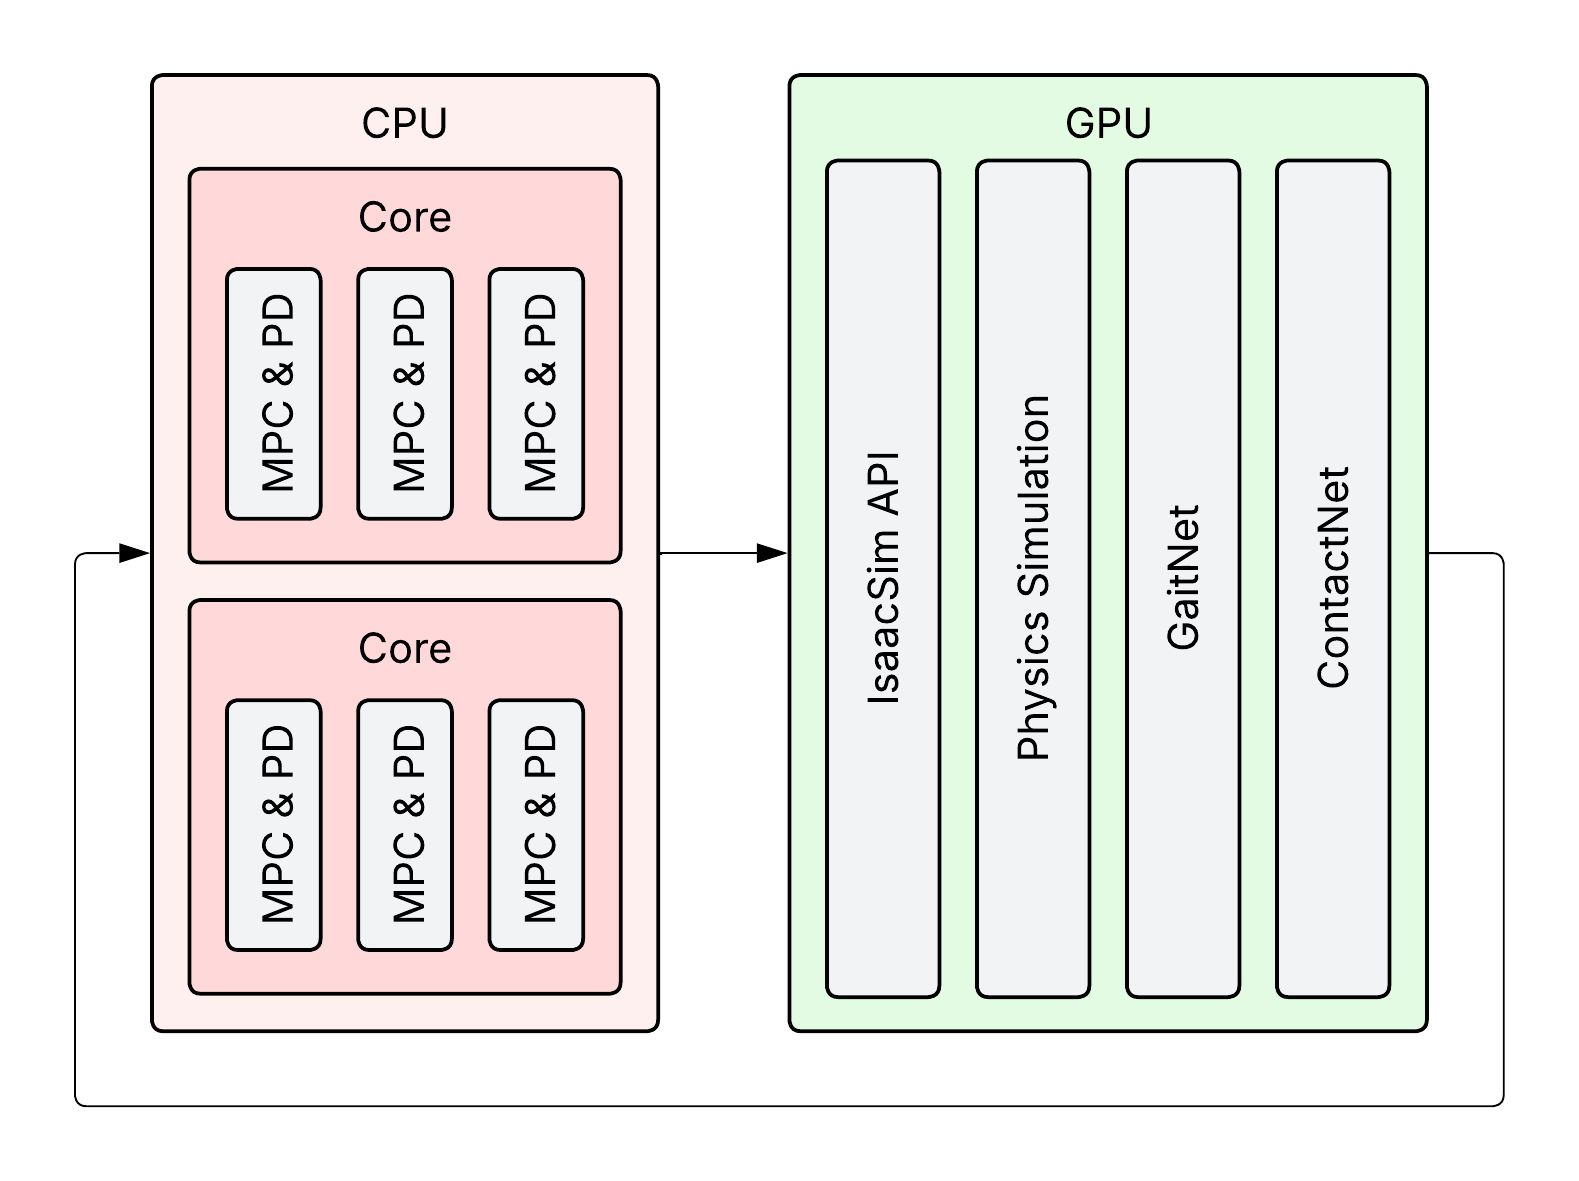
\includegraphics[width=0.5\linewidth]{images/diagrams/processing-flow.png}
  \caption{A block diagram showing the programming tasks computed on
    the CPU vs GPU. The full simulation is run in parallel using Nvidia
  Isaac Lab on the GPU, while the robot MPCs are run in parallel on the CPU.}
  \label{fig:diagram-processing-flow}
\end{figure}

NVIDIA Isaac Lab uses a declarative system of python dataclasses to
define the simulation environment. For this work, a custom
environment is used (\autoref{fig:figure-terrain-raycast}), including:

\begin{todo}
  update
\end{todo}

\begin{itemize}
  \item Unitree Go 1\textemdash Configured to use force control for each joint.
  \item Terrain raycasts\textemdash Measure the height of the terrain
    at each possible footstep location. This emulates the lidar
    processing steps of a full vision pipeline.
  \item Custom terrain\textemdash Planar terrain with sections
    missing on a grid pattern. The underlying grid is 8cm square, and
    the void density is tuned to create a challenging but possible
    environment. Multiple difficulty levels of the terrain are generated
    for the robots to progress through as they learn.
    The terrain is designed to mirror that used in
    \cite{bratta_contactnet_2024}
    through as they learn.
\end{itemize}

\begin{todo}
  update \autoref{fig:figure-terrain-raycast}
\end{todo}

\begin{figure}[H]
  \centering
  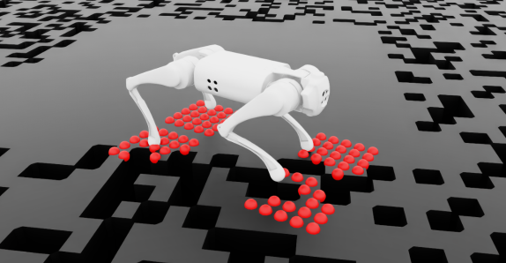
\includegraphics[width=0.75\linewidth]{images/figures/terrain-raycast.png}
  \caption{Image of a Unitree Go 1 navigating the terrain. Red
    spheres show the hit location of raycasts. Black regions show voids
  in the terrain.}
  \label{fig:figure-terrain-raycast}
\end{figure}
